%----------------------------------------------------------------------------------------
% Cadenas de Márkov
%----------------------------------------------------------------------------------------

En esta práctica se implementarán funciones para realizar cálculos básicos sobre cadenas de Márkov.

\section{Objetivo}

\begin{compactitem}
 \item Que el alumno se familiarice con los procesos estocásticos discretos denominados Cadenas de Márkov discretas y realice una implementación para resolver algunas de las preguntas más frecuentes que se pueden plantear sobre estos procesos. \parencite{gestiondeoperaciones2015}
\end{compactitem}


\section{Introducción}

\begin{figure}
 \centering
 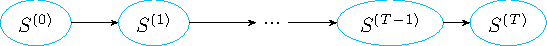
\includegraphics[width=0.8\textwidth]{markov/CadenaDeMarkov}
 \caption{Una Cadena de Márkov es una Red de Bayes degenerada.}\label{Fig:CadenaDeMarkov}
\end{figure}

\begin{definition}[Cadena de Márkov discreta]
 \begin{itemize}
  \item Una \emph{Cadena de Márkov} es un modelo bayesiano dinámico donde cada nodo representa el estado del sistema al tiempo $t$, denotado $S^{(t)}$, y éste sólo tiene un padre: el estado del sistema en el tiempo anterior $S^{t-1}$. [\fref{Fig:CadenaDeMarkov}]

  \item El sistema tiene un conjunto finito de estados discretos posibles $S = \{s_1,...,s_n\}$

  \item Asume \emph{invarianza temporal}, es decir, la probabilidad de transición $P(S^{(t+1)}|S^{(t)})$ es la misma para todo $t$.
 \end{itemize}
\end{definition}

\subsection{Inferencia}

Frecuentemente la probabilidad de transición de un estado a otro se expresa con un autómata al plantear el problema.  De este autómata es posible extraer el factor representando la probabilidad condicionar $P(S^{(t+1)}|S^{(t)})$, con las variables $S^{(t)}$ y  $S^{(t+1)}$ en su alcance.

Si a esto agregamos el factor con la distribución de probabilidad para el estado inicial $P(S^{(0)})$, es posible obtener $P(S^{(t)})$ para cualquier $t$ utilizando la regla de la cadena de Bayes.  Por ejemplo, para $t=1$:
\begin{align*}
 P(S^{(1)}) = \sum_{S^{(0)}} P(S^{(1)}|S^{(0)}) P(S^{(0)})
\end{align*}
con lo que obtenemos la probabilidad del que el sistema se encuentre en cualquier estado al tiempo $t=1$, independientemente de en qué estado haya iniciado.

Recursivamente:
\begin{align*}
 P(S^{(t+1)}) = \sum_{S^{(t)}} P(S^{(t+1)}|S^{(t)}) P(S^{(t)})
\end{align*}

Sin embargo, utilizar factores puede ser un cañón para este caso, pues cada nodo sólo tiene un nodo padre.  Podemos notar que la multiplicación de factores y marginalización sobre la variable padre, se pueden realizar en una sola operación si escribimos la distribución de probabilidad condicional en una matriz:
\begin{align*}
 T &= \begin{bmatrix}
        P(S=s_1|S=s_1) & ... & P(S=s_1|S=s_n) \\
        P(S=s_2|S=s_1) & ... & P(S=s_2|S=s_n) \\
        ... \\
        P(S=s_n|S=s_1) & ... & P(S=s_n|S=s_n) \\
       \end{bmatrix} \\
\end{align*}
y la distribución de probabilidad para el estado en cada tiempo con un vector:
\begin{align*}
  P(S) &= \begin{bmatrix}
	  P(s_1) \\
	  P(s_2) \\
	  ...\\
	  P(s_n)
	 \end{bmatrix}
\end{align*}
Entonces el cálculo de la distribución de probabilidad para otros tiempos se resume como:
\begin{align*}
 P(S^{t+1}) &= T P(S^{t}) \\
 P(S^{t+1}) &= T^n P(S^{0})
\end{align*}


\subsection{Ejemplo: El soldado}

Supongamos que estamos modelando el comportamiento de un soldado en un videojuego de acción.  Este soldado está vigilando un área restringida y puede tener alguno de tres comportamientos: estar caminando, quedarse de pie o dormido.  El estado del soldado queda descrito por la variable $S \in \{caminando, dormido, de\ pie\}$, lo cual en ocasiones abreviaremos como $S \in \{cam, dor, d.p.\}$.  Para que su comportamiento no sea tan predecible, cambiará su actividad aleatoriamente según describe el autómata en la \fref{Fig:SoldadoMarkov}.

\begin{figure}
 \centering
 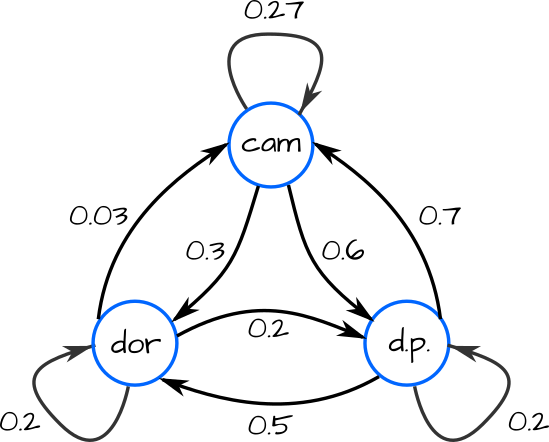
\includegraphics[width=0.4\textwidth]{markov/SoldadoMarkov}
 \caption{Las probabilidades de transición expresadas con un autómata.}\label{Fig:SoldadoMarkov}
\end{figure}

Entonces, la matriz de transición se acomoda como en la tabla siguiente:

 \begin{center}
 \begin{tabular}{l|ccc}
  \multicolumn{4}{c}{$P(S^{(t+1)}|S^{(t)})$} \\ \hline
  $S^{(t+1)}$ \textbackslash $S^{(t)}$          & caminando & dormido & de pie \\ \hline
  caminando &    0.27   &    0.3  & 0.6 \\
  dormido   &    0.03   &    0.2  & 0.2 \\
  de pie    &    0.7    &    0.5  & 0.2
 \end{tabular}
 \end{center}

 Inicialmente sea:

 \begin{center}
 \begin{tabular}{l|c}
  \multicolumn{1}{c|}{$S^{(0)}$}   &  $P(S^{(0)})$ \\ \hline
  caminando &    0.2 \\
  dormido   &    0.2 \\
  de pie    &    0.6
 \end{tabular}
 \end{center}

Para calcular qué es probable que esté haciendo el soldado al tiempo siguiente basta con multiplicar:
\begin{align*}
 P(S^{(1)}) &= T P(S^{(0)}) \\
   &= \begin{bmatrix}
        0.27 & 0.3 & 0.6 \\
        0.03 & 0.2 & 0.2 \\
        0.7  & 0.5 & 0.2
       \end{bmatrix}
       \begin{bmatrix}
	    0.2 \\
	    0.2 \\
	    0.6
	 \end{bmatrix} \\
   &=  \begin{bmatrix}
        0.474 \\
        0.166 \\
        0.36
       \end{bmatrix}
\end{align*}

\subsection{Estado estacionario}

\begin{definition}[Cadena irreducible]
 Se dice que una cadena es \emph{irreducible} si es posible acceder a cualquier estado desde cualquier otro estado, ya sea directamente o a través de un camino de nodos.
\end{definition}

\begin{definition}[Estado periódico]
 ``Un estado es periódico si, partiendo de ese estado, sólo es posible volver a él en un número de etapas que sea múltiplo de un cierto número entero $d$ mayor que uno.''

 ``Si $d = 1$ decimos que el estado es \emph{aperiódico}.''
 \parencite{gestiondeoperaciones2013}
\end{definition}

En particular, un sistema donde es posible transitar desde un estado $s_i$ a cualquier otro estado $s_j$ directamete, da lugar a una cadena irreducible con estados aperiódicos.  Cuando estas dos condiciones se cumplen, la cadena eventualmente alcanzará un \emph{estado estacionario}, donde la distribución de probabilidad al tiempo $t+1$ será igual a la distribución al tiempo $t$.  Es decir, cumple con la ecuación:
\begin{align*}
 P(S^{(t)}) &= T P(S^{(t)})
\end{align*}

Adicionalmente, como se trata de una distribución de probabilidad, las componentes de $P(S)$ deben sumar uno:
\begin{align*}
 \sum_i P(s_i) &= 1
\end{align*}

Si el número de valores posibles para $S$ es $n$, esto nos da un sistema de $n+1$ ecuaciones linealmente independientes.  Este sistema está sobre determinado, por lo que para resolverlo se realiza una aproximación utilizando mínimos cuadrados \parencite{Maplesoft2022}.

El sistema en forma matricial se escribe:
\begin{align*}
 (T - \mathbb{1})P(S^{(t)}) &= \mathbb{0} \\
 [1 1 ... 1]P(S^{(t)}) &= 1
\end{align*}
Concatenando los renglones de ambas matrices:
\begin{align*}
 \begin{bmatrix}
   T - \mathbb{1} \\
   1 1 ... 1
 \end{bmatrix}
 P(S^{(t)}) &=
 \begin{bmatrix}
  \mathbb{0} \\
  1
 \end{bmatrix}
\end{align*}

Mínimos cuadrados ajustará un plano que pase lo más cerca posible de los puntos descritos por cada renglón de la matriz que multiplica a $P(S^{(t)})$.


\subsection{Ejemplo: comportamiento del soldado en el estado estacionario}

Si bien el comportamiento del soldado de nuestro ejemplo mutará más al inicio, eventualmente se estabilizará en una rutina donde una sola distribución de probabilidad describirá qué podría estar haciendo.  Para encontrar esta distribución el sistema que debemos resolver ajustando mínimos cuadrados es:
\begin{align*}
 \begin{bmatrix}
  -0.73 & 0.3  & 0.6 \\
   0.03 & -0.8 & 0.2 \\
   0.7  &  0.5 & -0.8 \\
   1    &  1   &  1
 \end{bmatrix}
 \begin{bmatrix}
  cam \\
  dor \\
  d.p.
 \end{bmatrix} &=
 \begin{bmatrix}
  0 \\
  0 \\
  0 \\
  1
 \end{bmatrix}
\end{align*}

El resultado es:
\begin{align*}
 P(S) &= \begin{bmatrix}
  0.42220485 \\
  0.12822518 \\
  0.44956998
 \end{bmatrix}
\end{align*}
y es posible verificar que $TP = P$.

La \fref{fig:MinimosCuadrados} muestra los puntos descritos por esta matriz y el plano definido por la solución encontrada.

\begin{figure}
 \centering
 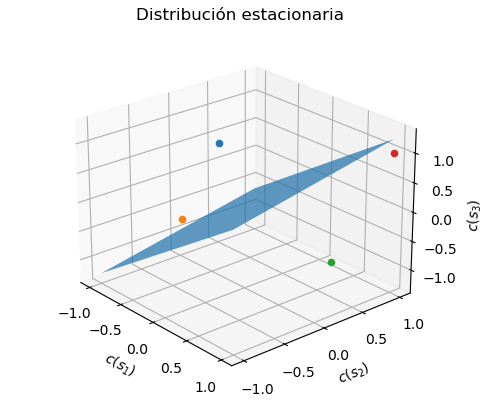
\includegraphics[width=0.6\textwidth]{markov/MinimosCuadrados}
 \caption{El plano ajustado corresponde a la distribución estacionaria.}\label{fig:MinimosCuadrados}
\end{figure}


Hay más consultas que se pueden realizar con una cadena de Márkov, con los conocimientos que tienes de redes de Bayes ya te debe ser posible inferir lo que tienes que hacer.  Si aún tienes dudas puedes consultar la página sobre cadenas de Márkov en \hurl{https://en.wikipedia.org/wiki/Markov_chain} así como algunos ejemplos sencillos en \hurl{https://en.wikipedia.org/wiki/Examples_of_Markov_chains}.



\section{Desarrollo}

Para esta práctica se requiere implementar una clase para trabajar con cadenas de Márkov.  Se recomienda programarla en \code{Python}, ya que la biblioteca \code{numpy} contiene métodos para trabajar con matrices y vectores, lo cual simplifica mucho los puntos siguientes.  También se recomienda utilizar matrices columna para representar vectores, de esta manera funcionarán correctamente las multiplicaciones de matriz por vector.

La clase \code{CadenaDeMarkov} debe contener:

\begin{enumerate}
 \item Un constructor que reciba como parámetros:
 \begin{enumerate}
  \item Una lista con los nombres los estados posibles.
  \item Un vector con la probabilidad de iniciar en cada uno de los estados posibles.
  \item Una matriz de probabilidades, con la probabilidad de transitar de cada estado hacia los demás.
 \end{enumerate}

 \item Un método para generar una secuencia de estados a partir del modelo de Márkov iniciado dado el número $n$ de elementos que tendrá la secuencia; opcionalmente puede recibir como parámetro una semilla para la generación de números aleatorios.
 
 Para generar esta muestra necesitarás calcular los vectores con las distribuciones de probabilidad para $n$ pasos.  Dada cada distribución, utiliza un número aleatorio para determinar cuál de los estados corresponderá a ese paso.
 
 Devuelve una lista con la secuencia de estados.
 
 \item Obtener la probabilidad de una cadena de estados (punto extra si se permite que esta cadena tenga estados indeterminados).  Observa que esta es la distribución de probabilidad conjunta $P(S_0=s_0,S_1=s_1,...,S_n=s_n)$, escrito de otra forma, $P(s_0,s_1,...,s_n)$.  Deberá recibir como parámetro una lista con la secuencia de estados y devolver la probabilidad.
 
 \item Estimar las probabilidades a largo plazo de cada uno de los estados, es decir, la distribución límite, cuando sea posible.  Este método deberá devolver el vector con la distribución de probabilidades.
 
 \item Agregar un archivo donde se utilice tu clase para resolver un ejemplo, usando cada uno de los métodos.  Puedes usar algún ejemplo del sitio de gestión de operaciones.
\end{enumerate}


\subsection{Requisitos y resultados}

Incluir:

\begin{enumerate}
 \item El archivo de la clase \code{CadenaDeMarkov}.
 \item El archivo con el demo de prueba.
\end{enumerate}

